\chapter{Resultados de 10 ejecuciones con política M-Armed-Bandit}
\label{resultBandit10}

Los datos de entrada que arrojaron estos resultados son los mismos que se utilizron en ejecuciones anteriores, para poder realizar el comparativo correspondiente.

De acuerdo a la teoría de Aprendizaje por Refuerzo, el jugador de M-Armed-bandit, no conoce el valor real de cada bandit, pero va recibiendo recompensas o castigos que le pueden ayudar a descubrir, no la ganancia exacta de cada uno, pero sí, cuál tiene la mejor ganancia. Esto se consigue haciendo un promedio de esas recompensas, para cada uno de los bandit y al final escogiendo el que tenga el mejor promedio.

Ese es el principio que se quiso seguir en la escogencia de la ruta óptima es este ejercicio, seleccionar la mejor ganancia promedio, cuyo argumento se constituye en un arreglo de nodos con longitud igual a la cantidad de etapas dadas, lo que no facilitó el desarrollo. Pero, de acuerdo al archivo que aquí se anexa, de 10 ejecuciones que se hacen continuas del algoritmo, 10 convergen a la respuesta deseada, lo cual, al menos para problemas sencillos como el del ejemplo, es un buen resultado.

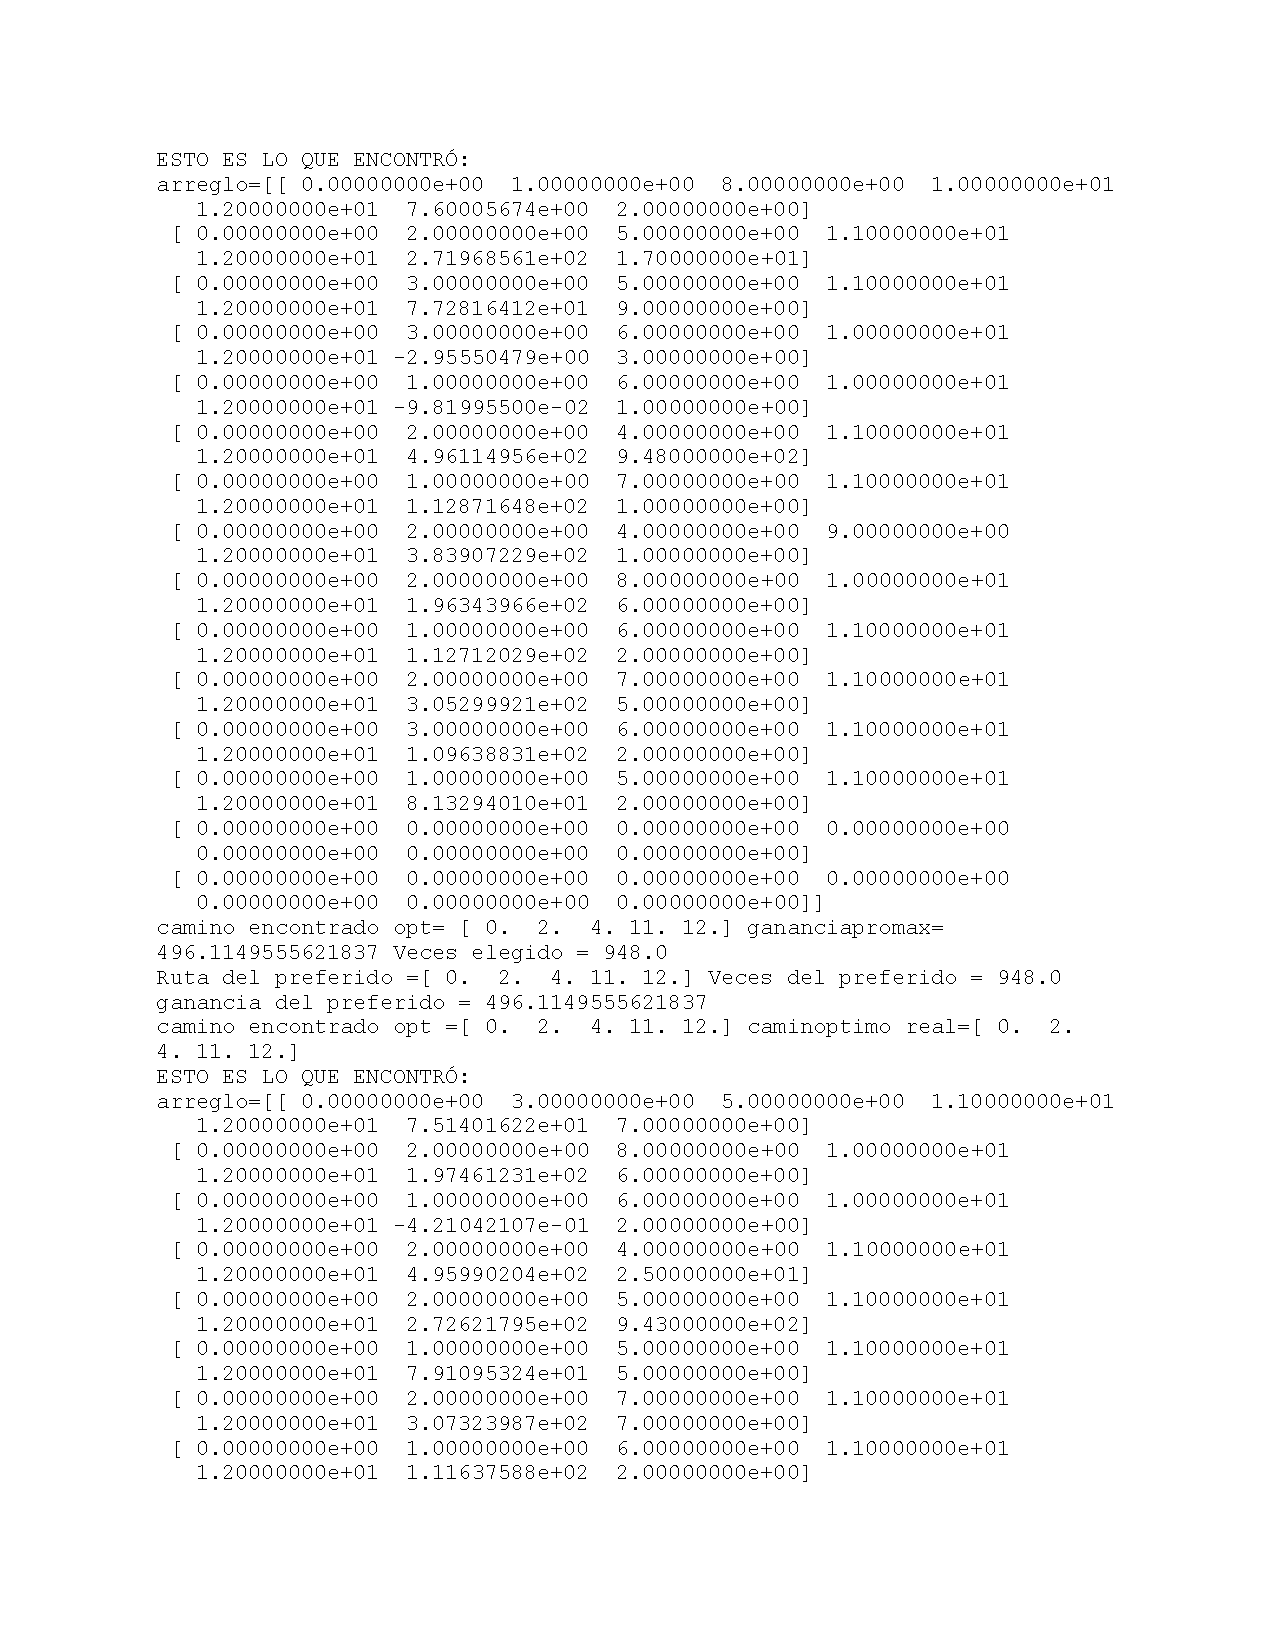
\includepdf[pages=-]{ResultMBandit}